\documentclass[12pt,a5paper,openany]{memoir}
\raggedbottom

\usepackage{geometry}
\geometry{
  a5paper,
  top=8mm,
  left=18mm,
  right=21mm,
  bottom=10mm,
%  showframe,
}
\usepackage{fontspec}
\usepackage{titlesec}
\usepackage{xcolor}
\usepackage{enumitem}
\usepackage[defaultlines=5,all]{nowidow}
\usepackage[pdfusetitle,colorlinks=true]{hyperref}
\usepackage{float}
\usepackage{graphicx}
\usepackage{wrapfig}
\usepackage{marginnote}
\usepackage{amssymb}

%% Page style
\makepagestyle{songs}
% Hack: Right pagination is moved right by using the margin
\makeoddfoot{songs}{}{}{\marginnote{\hspace{2mm}$\langle$\thepage$\rangle$}}
% Hack: Left pagination is moved left with a kern
\makeevenfoot{songs}{\kern-8mm$\langle$\thepage$\rangle$}{}{}
% Patch cleardoublepage to not get blank pages after title & contents pages:
\renewcommand\cleardoublepage{\clearpage}

%% Fonts and colours
% This file is used by the generated TeX file for font settings.
% Note that the Path here is relative to the `output` directory
% rather than `output/fonts` because that's where the .tex file is generated.

\setromanfont{DroidSerif}[
    Path = ./fonts/,
    Extension = .ttf,
    UprightFont = *-Regular,
    BoldFont = *-Bold,
    ItalicFont = *-Italic,
    BoldItalicFont = *-BoldItalic
]

\setsansfont{NotoSans}[
    Path = ./fonts/,
    Extension = .ttf,
    UprightFont = *-Regular,
    BoldFont = *-Bold,
    ItalicFont = *-Italic,
    BoldItalicFont = *-BoldItalic
]

\colorlet{LightRed}{red!65!}
\colorlet{DarkGray}{black!70!}

%% Spacings
\setlength{\parindent}{0pt}
\setlength{\tabcolsep}{0pt}
\setlength{\parskip}{1mm}
\setlength{\footskip}{2mm}

%% ToC style
% Suppress page numbers
\aliaspagestyle{chapter}{empty}
% Hide the title of the ToC:
\renewcommand\tocheadstart{}
\renewcommand\printtoctitle[1]{}
\renewcommand\aftertoctitle{}
% Hide section numbers in the ToC:
\renewcommand\numberline[1]{}
\renewcommand\cftdotsep{1}

%% Hyperlinks setup
\hypersetup{
  bookmarks=true,
  linkcolor=.,
  urlcolor=blue,
  pdfcreator=bard v. 1.3.0 - https://github.com/vojtechkral/bard,
}

%% Song title and subtitle formats
\titleformat{\section}
  {\large\bfseries}{}{0pt}{\underline}
\titlespacing*{\section}
  {0pt}{7mm}{0pt}
\newcommand\songtitle[1]{%
  % This is a trick to only layout a song on the current page
  % if it fits, otherwise a pagebreak is inserted
  \FloatBlock
  \vfil
  \pagebreak[2]
  \vfilneg
  \section{#1}
}
\newcommand\subtitle[1]{%
  \emph{#1}
}

%% Verse layout command
\makeatletter
% The verse & label layout code was written by Jonathan P. Spratte
% under the Beerware license: As long as you retain this notice you
% can do whatever you want with this stuff. If we meet some day, and you think
% this stuff is worth it, you can buy me a beer in return. Jonathan P. Spratte
\newlength\verse@indent
\newlength\verse@labelsep
\newlength\verse@vskip
\AtBeginDocument{% setting AtBeginDocument since earlier we can't rely on em being correct
  \verse@indent=9mm
  \verse@labelsep=1mm
  \verse@vskip=\smallskipamount
}
\newcommand\Verse[1]{%
    \par
    \vskip\verse@vskip
    \noindent\kern-\verse@indent
    \sbox0{\textbf{\footnotesize{#1}}}%
    \ifdim\wd0>\dimexpr\verse@indent-\verse@labelsep\relax
      \usebox0\kern\verse@labelsep
    \else
      \makebox[\verse@indent]{\usebox0}%
    \fi
    \ignorespaces
}
\makeatother
























% Metadata
\title{Test Songbook}

% Document
\begin{document}

%% Title page
\frontmatter*
\newgeometry{margin=5mm}
\begin{titlingpage*}
  \begin{vplace}[0.5]
    \begin{center}
      \Huge{\textbf{Test Songbook}} \\
      \vspace{0.5cm}
      \LARGE{Exercising all features} \\
        \vspace{1cm}
        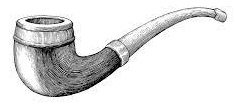
\includegraphics[width=41.451388888888886mm]{pipe.jpg}
    \end{center}
  \end{vplace}

  \mbox{}
  \vfill
  \begin{center}\small{Hopefully all features}\end{center}
\end{titlingpage*}
\restoregeometry

%% Contents page
\pagestyle{empty} % Suppresses ToC continuation page header
\tableofcontents*

%% Songs
\mainmatter*

\pagestyle{songs}
  %% song 0
  \songtitle{Danny Boy}

\subtitle{English ballad}\\\subtitle{Subtitle 2}
    \vspace{2mm}
  

  \Verse{} This~is~an~unlabeled~verse.

    \vspace{\parskip}

\Verse{Intro} \begin{tabular}[b]{l}
    \textbf{\sffamily\color{red}{G7~C~C7~F}}\mbox{}\end{tabular}

    \vspace{\parskip}

\Verse{1.} \begin{tabular}[b]{l}
    \textbf{\sffamily\color{red}{A7}}\\
    \textbf{\sffamily\color{red}\color{blue}{I7}}\\Oh~\textbf{Danny}~\mbox{}\end{tabular}\begin{tabular}[b]{l}
    \textbf{\sffamily\color{red}{D}}\\
    \textbf{\sffamily\color{red}\color{blue}{IV}}\\Boy,~the~\emph{pipes},~the~\mbox{}\end{tabular}\begin{tabular}[b]{l}
    \small{\sffamily\color{LightRed}{D7}}\\
    \small{\sffamily\color{LightRed}\color{blue}{IV7}}\\pipes~are~\mbox{}\end{tabular}\begin{tabular}[b]{l}
    \textbf{\sffamily\color{red}{G}}\\
    \textbf{\sffamily\color{red}\color{blue}{VIIb}}\\calling\mbox{}\end{tabular}\\
From~\href{https://en.wikipedia.org/wiki/Glen}{glen}~to~\begin{tabular}[b]{l}
    \textbf{\sffamily\color{red}{D}}\\
    \textbf{\sffamily\color{red}\color{blue}{IV}}\\glen,~and~\mbox{}\end{tabular}\begin{tabular}[b]{l}
    \textbf{\sffamily\color{red}{F\#m}}\\
    \textbf{\sffamily\color{red}\color{blue}{VIm}}\\down~the~\mbox{}\end{tabular}\begin{tabular}[b]{l}
    \textbf{\sffamily\color{red}{G}}\\
    \textbf{\sffamily\color{red}\color{blue}{VIIb}}\\mountain~\mbox{}\end{tabular}\begin{tabular}[b]{l}
    \textbf{\sffamily\color{red}{A7}}\\
    \textbf{\sffamily\color{red}\color{blue}{I7}}\\side\mbox{}\end{tabular}\\
The~summer’s~\begin{tabular}[b]{l}
    \textbf{\sffamily\color{red}{D}}\\
    \textbf{\sffamily\color{red}\color{blue}{IV}}\\gone,~and~all~the~\mbox{}\end{tabular}\begin{tabular}[b]{l}
    \small{\sffamily\color{LightRed}{D7}}\\
    \small{\sffamily\color{LightRed}\color{blue}{IV7}}\\flowers~are~\mbox{}\end{tabular}\begin{tabular}[b]{l}
    \textbf{\sffamily\color{red}{G}}\\
    \textbf{\sffamily\color{red}\color{blue}{VIIb}}\\dying\mbox{}\end{tabular}\\
\emph{‘Tis~you,~\textbf{’tis~}}\begin{tabular}[b]{l}
    \textbf{\sffamily\color{red}{D}}\\
    \textbf{\sffamily\color{red}\color{blue}{IV}}\mbox{}\end{tabular}\emph{\textbf{~you~must}~}\begin{tabular}[b]{l}
    \textbf{\sffamily\color{red}{Em}}\\
    \textbf{\sffamily\color{red}\color{blue}{Vm}}\\\emph{go~and~}\mbox{}\end{tabular}\begin{tabular}[b]{l}
    \textbf{\sffamily\color{red}{A7}}\\
    \textbf{\sffamily\color{red}\color{blue}{I7}}\\\emph{I~must~}\mbox{}\end{tabular}\begin{tabular}[b]{l}
    \textbf{\sffamily\color{red}{D}}\\
    \textbf{\sffamily\color{red}\color{blue}{IV}}\\\emph{bide.}\mbox{}\end{tabular}

    \vspace{\parskip}

\Verse{Ch1.} \begin{tabular}[b]{l}
    \textbf{\sffamily\color{red}{6b7}}\\But~come~ye~\mbox{}\end{tabular}\begin{tabular}[b]{l}
    \textbf{\sffamily\color{red}{7bm}}\\back~when~\mbox{}\end{tabular}\begin{tabular}[b]{l}
    \textbf{\sffamily\color{red}{4\#}}\\summer’s~\mbox{}\end{tabular}\begin{tabular}[b]{l}
    \textbf{\sffamily\color{red}{6b7}}\\in~the~\mbox{}\end{tabular}\begin{tabular}[b]{l}
    \textbf{\sffamily\color{red}{1\#}}\\meadow\mbox{}\end{tabular}\\
Or~when~the~\begin{tabular}[b]{l}
    \textbf{\sffamily\color{red}{7bm}}\\valley’s~\mbox{}\end{tabular}\begin{tabular}[b]{l}
    \textbf{\sffamily\color{red}{4\#}}\\hushed~and~\mbox{}\end{tabular}\begin{tabular}[b]{l}
    \textbf{\sffamily\color{red}{4m}}\\white~with~\mbox{}\end{tabular}\begin{tabular}[b]{l}
    \textbf{\sffamily\color{red}{3b7}}\\snow~\mbox{}\end{tabular}\begin{tabular}[b]{l}
    \textbf{\sffamily\color{red}{6b7}}\\\mbox{}\end{tabular}\\
‘Tis~I’ll~be~\begin{tabular}[b]{l}
    \textbf{\sffamily\color{red}{1\#}}\\here~in~\mbox{}\end{tabular}\begin{tabular}[b]{l}
    \textbf{\sffamily\color{red}{4\#}}\mbox{}\end{tabular}~sunshine~or~in~\begin{tabular}[b]{l}
    \textbf{\sffamily\color{red}{1\#}}\\sha\mbox{}\end{tabular}\begin{tabular}[b]{l}
    \textbf{\sffamily\color{red}{7bm}}\\dow.\mbox{}\end{tabular}\\
Oh~Danny~\begin{tabular}[b]{l}
    \textbf{\sffamily\color{red}{1\#}}\\Boy,~oh~Danny~\mbox{}\end{tabular}\begin{tabular}[b]{l}
    \textbf{\sffamily\color{red}{4\#}}\\Boy,~I~\mbox{}\end{tabular}\begin{tabular}[b]{l}
    \textbf{\sffamily\color{red}{6b7}}\\love~you~\mbox{}\end{tabular}\begin{tabular}[b]{l}
    \textbf{\sffamily\color{red}{1\#}}\\so.\mbox{}\end{tabular}

    \vspace{\parskip}

\Verse{Second verse} \\
And~if~you~come,~    \hfill\hspace{0pt}\vspace{-1em}
    {
    \begin{wrapfigure}{r}{41.451388888888886mm}
      \centering
      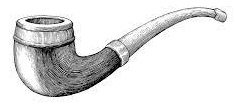
\includegraphics[width=41.451388888888886mm]{pipe.jpg}
    \end{wrapfigure}
    }
\\
when~all~the~flowers~are~dying\\
And~I~am~dead,\\
As~dead~I~well~may~be\\
You’ll~come~and~find\\
The~place~where~I~am~lying\\
And~kneel~and~say~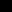
\includegraphics[width=2.1166666666666663mm]{box.png}~an~”Ave”~there~for~me.

    \vspace{\parskip}

\begin{itemize}[noitemsep]\item Bullet list item 1
\item Bullet list item 2
  \end{itemize}
\Verse{Ch2.} And~I~shall~hear,~though~soft~you~tread~above~me\\
And~all~my~dreams~will~warm~and~sweeter~be

    \vspace{\parskip}

  \vphantom{}\hrule
\Verse{} If~you’ll~not~fail~to~tell~me~that~you~love~me\\
I’ll~sleep~in~peace~until~you~come~to~me.

    \vspace{\parskip}

 
    \begin{figure}[H]
      \centering
      \includegraphics[width=102.30555555555554mm]{hills.jpg}
    \end{figure}



    \vspace{\parskip}


  %% song 1
  \songtitle{Wildcard 1}

  \vspace{2mm}{}

  \Verse{Ch.} \begin{tabular}[b]{l}
    \textbf{\sffamily\color{red}{Am}}\\Yippie~yea~\mbox{}\end{tabular}\begin{tabular}[b]{l}
    \textbf{\sffamily\color{red}{C}}\\oh!~Yippie~yea~\mbox{}\end{tabular}\begin{tabular}[b]{l}
    \textbf{\sffamily\color{red}{Am}}\\yay!\mbox{}\end{tabular}

    \vspace{\parskip}


  %% song 2
  \songtitle{Wildcard 2}

  \vspace{2mm}{}

  \Verse{1.} \begin{tabular}[b]{l}
    \textbf{\sffamily\color{red}{Am}}\\Yippie~yea~\mbox{}\end{tabular}\begin{tabular}[b]{l}
    \textbf{\sffamily\color{red}{C}}\\oh!~Yippie~yea~\mbox{}\end{tabular}\begin{tabular}[b]{l}
    \textbf{\sffamily\color{red}{Am}}\\yay!\mbox{}\end{tabular}

    \vspace{\parskip}


  %% song 3
  \songtitle{Multiple Songs 1}

  \vspace{2mm}{}

  \Verse{1.} \begin{tabular}[b]{l}
    \textbf{\sffamily\color{red}{Am}}\\Yippie~yea~\mbox{}\end{tabular}\begin{tabular}[b]{l}
    \textbf{\sffamily\color{red}{C}}\\oh!~Yippie~yea~\mbox{}\end{tabular}\begin{tabular}[b]{l}
    \textbf{\sffamily\color{red}{Am}}\\yay!\mbox{}\end{tabular}

    \vspace{\parskip}


  %% song 4
  \songtitle{Multiple Songs 2}

  \vspace{2mm}{}

  \Verse{1.} \begin{tabular}[b]{l}
    \textbf{\sffamily\color{red}{Am}}\\Yippie~yea~\mbox{}\end{tabular}\begin{tabular}[b]{l}
    \textbf{\sffamily\color{red}{C}}\\oh!~Yippie~yea~\mbox{}\end{tabular}\begin{tabular}[b]{l}
    \textbf{\sffamily\color{red}{Am}}\\yay!\mbox{}\end{tabular}

    \vspace{\parskip}



\backmatter

\end{document}
